\documentclass[10pt,a4paper]{article}
\usepackage{graphicx}
\usepackage{apacite}
\usepackage{amsmath}   
\usepackage{caption}
\usepackage{subcaption} 
\usepackage{algorithm}
\usepackage[noend]{algpseudocode}


\newtheorem{assumption}{Assumption}
\usepackage{enumitem}
\newlist{steps}{enumerate}{1}
\setlist[steps, 1]{label = Step \arabic*:}


\begin{document}

\section{Global Nearest Neighbour: Algorithmus und Idee}
\section{Grundlage \textit{GNN}}
Da die Verfolgung der exakten gesuchten posteriori Wahrscheinlichkeit, aufgrund begrenzter Rechnerzeit und hohen Rechneraufwand, nicht genau bestimmbar ist, sind Approximationen für eine durchführbare Rechnung erforderlich. In diesem Kapitel wird der einfachste und rechnengünstigste Tracking Algorithmus vorgestellt, der Global Nearest Neighbour (\textit{GNN}).\\
Wie bereits erwähnt, werden hauptsächlich zwei Annahmen getroffen, um die Problematik noch berechenbar zu gestalten, die sogenannte Merging und Pruning. Der \textit{GNN} basiert sich auf ein abruptes Pruning.
\subsection{Bekannte Anzahl von Objekten}
Eine wichtige Annahme und gleichzeitig Einschränkung dieses Algorithmus, bezieht sich auf die Voraussetzung, dass die Anzahl der Objekte $n_k$ in jedem Zeitschritt bekannt ist. Diese Annahme ist hinsichtlich einer Performance Analyse auf künstliche Testdaten ausreichend, allerdings wird der Algorithmus für eine Realitätsnahe Simulation so gut wie unbrauchbar. In den späteren Kapiteln, wird die \textit{M/N} Methode vorgestellt, die eine Einschätzung von $n_k$ liefern kann, daher wäre der GNN bei einer praktischen Anwendung verwendbar.
\subsection{Pruning in dem \textit{GNN} Context}
Hinsichtlich der Übersichtlichkeit der vorhanden Problematik, stellt man sich folgendes Szenario vor: Bei jedem Zeitschritt $k$ (immer wenn ein neues Bild aufgenommen wird), erhält der Algorithmus verschiedenen Messungen $\underline{z}_k$ mit x und y Koordinaten aus der Objektdetektion. Dies enthält sowohl Clutters wie die Koordinaten der echten Objekten. Ohne eine genauere Analyse, sind diese beiden Größen nicht unterscheidbar, daher bewertet man über Zeitschritten hinweg, welche der Koordinaten näherungsweise einem \textit{Constant Velocity Model} entsprechen können. Je mehr die Reihe der Koordinaten einer konstanten Geschwindigkeit Annahme folgt, desto wahrscheinlicher ist es, dass es sich um ein echtes Objekt handelt. Auf der anderen Seite, Reihen von 
Koordinaten deren vorkommen zufällig erscheinen, werden mit höherer Wahrscheinlich den Clutters zugewiesen. Wir definieren $m_k$ als die gesamte Anzahl der Koordinaten der echten Objekte und Koordinaten der Clutters.\\
Eine Datenanalyse ohne das Pruning, müsste alle mögliche Kombinationen der Daten bewerten. Zum Beispiel für lediglich zwei Zeitschritten $k =0$ und $k=1$ mit jeweiligen zwei Messungen  $m_0 = 2$ und $m_1 = 2$, entstehen 4 Assoziationsmöglichkeiten, da sowohl die erste, wie die zweite Koordinate von der Messung $z_0$ zwei Alternativen besitzen sich mit den Koordinaten der $z_1$ zu Assoziieren.\\
Laut \cite{MOTyoutube} die Gleichung, die die gesamte Anzahl aller Assoziationen $N_A$ für beliebige Objektanzahl $n_k$ und beliebige Messungen $m_k$ vorgibt lautet:
\begin{equation}
N_A(m_k,n_k) = \sum_{\delta=0}^{min(m_k,n_k)}\dfrac{m_k!n_k!}{\delta!(m_k-\delta)!(n_k-\delta)!}
\end{equation}
Infolge dessen, für $m_k=n_k = 8$, entstehen bereits 1441729 mögliche Assoziationen. Dieses Beispiel vermittelt wie wesentlich für den Rechneraufwand es sei, die Hypothesen Anzahl mithilfe des Prunings einzuschränken. \\
Bei dem \textit{GNN}, wird lediglich die wahrscheinlichste Assoziation beibehalten, alle anderen möglichen Kombinationen werden bei jedem Zeitschritt \textit{weggeprunt}. Diese Eigenschaft verleiht dem \textit{GNN} die Schnelligkeit und Einfachheit, die seine Anwendung auf kosten der Genauigkeit gerechtfertigt. Aus dem Grund, dass nur die wahrscheinlichste Hypothese bei jedem Zeitschritt $k$ berücksichtigt wird, wird dieser Algorithmus als \textit{Greedy-Algorithm} bezeichnet. \\
Mithilfe des Prunings, kann man die folgenden posteriori Wahrscheinlichkeit der Objektzuständen $\underline{x_k}$ darstellen.
\begin{equation}
p_{k|k}^{GNN}(\underline{x_k}) = p_{k|k}^{\theta^*_{1:k}}(\underline{x_k}),
\end{equation} 
wo $\theta_k^*$ die wahrscheinlichste Assoziationshypothese repräsentiert. $\theta^*_{1:k}$ stellt eine Reihe von wahrscheinlichsten Assoziationshypothesen bis den Zeitschritt $k$ dar. Das Ziel wäre natürlich die posteriori Wahrscheinlichkeit für die jeweilige Objekte getrennt auszurechnen, also alle $p_{k|k}^{\theta^{*,i}_{1:k}}(\underline{x}_k^i)$ für $i = 1,...,n_k$.

\subsection{Allgemeine Vorgehensweise }
Mit einer bekannten Anzahl von Objekten $n_k$ und ohne weitere Vereinfachungen sind die Hauptschritte dieses Algorithmus folgendermaßen abgebildet.\\
Für jeden Zeitschritt $k$:\\
\begin{steps}\label{Stp:basicStepsGNN}
  \item \textbf{Prädiktion}\\
  Für jedes Objekt $i$, $p_{k|k-1}^{i}(\underline{x}_k^i)$  mithilfe einer Chapman-Kolmogorov Prädikation ausrechnen
  \item Wahrscheinlichste Hypothese ermitteln.
  \item \textbf{Update}\\
   Für jedes Objekt $i$, $p_{k|k}^{i}(\underline{x}_k^i)$  mithilfe eines Bayes-Update ausrechnen, falls das Objekt detektiert worden ist. Ansonsten $p_{k|k}^{i}(\underline{x}_k^i) = (1-P^D)p_{k|k-1}^{i}(\underline{x}_k^i)$. $P^D \in [0,1]$ sei die Detektionsrate und wird als Konstant angenommen.
   \item\label{step:erwartungsWert} Zustand aus der Aposteriori Wahrscheinlichkeit mithilfe des Erwartungswerts bestimmen \\
   $\underline{x}_k =  \int x_k^i p_{k|k}^{GNN}(\underline{x_k}) dx_k^i$
  
\end{steps}

\subsection{Unabhängige Objektzustände}
Da die vorherigen Schritte für eine reale Anwendung unpraktisch sein können, setzt man folgenden Annahmen voraus.

\begin{assumption}-\label{Ass:LinMod}
  Das Zustandsmodell sei linear.
\end{assumption}
\begin{assumption}-\label{Ass:ZustUnab}
  Die Objektzustände seien linear unabhängig.
\end{assumption}
\begin{assumption}-\label{AssGauss}
  Gauß'sche Wahrscheinlichkeitsdichte der Objektbewegung.
\end{assumption}
Seien Sie erfüllt, ist der Einsatz eines Kalman-Filters bei der Prädikation beziehungsweise dem Update möglich, was die Berechnung wesentlich vereinfacht. Außerdem, kann man sich auf die Berechnung auf \ref{step:erwartungsWert} verzichten, da eine direkte Ermittlung der Zustände ohne die Aposteriori Wahrscheinlichkeit möglich ist. Das nächste Kapital zeigt wie der Algorithmus mithilfe dieser Vereinfachungen aufgebaut wird.
\section{GNN Algorithmus}\label{subsec:GNNAlg}
\subsection{GNN Kalman-Filter}
Wenn die Voraussetzungen \ref{Ass:LinMod} bis \ref{AssGauss} des vorherigen Kapitels erfüllt sind, kann der GNN die Eigenschaften des Kalman-Filters ausnutzen. Dieses Filter handelt sich um einen Zustandsschätzer, der das Eingangs beziehungsweise Ausgangsrauschen eines dynamischen Systems minimieren kann. Dafür werden zwei Hauptschritten erforderlich: die Prädikation und die Korrektur (oder Update).\\
Das Kalman-Filter benötigt drei Parameter, die die Leistung der Schätzung stark beeinflussen können. Die positiv-definite Matrix der Varianz des Modellrauschens $\textbf{Q} \in \Re^{4x4}$, die positiv-definite Matrix der Varianz des Messrauschens $\textbf{R} \in \Re^{2x2}$ und letztlich die symmetrische  Objekt Kovarianzmatrix des Systemrauschens $\textbf{P}^i \in \Re^{2x2}$. Die Matrizen $\textbf{Q}$ und $\textbf{R}$ sind für alle Objekte gleich und Konstant. Matrix $\textbf{P}^i$ wird bei jedem Korrekturschritt aktualisiert und ist für die jeweilige Objekte $i$ unterschiedlich. Die Prädiktion und Korrektur werden bei jedem Zeitschritt erneut aufgerufen und sind für jedes Objekt $i = 1,...,n_k$ getrennt auszuführen. Der Einfluss der Wahl der Matrizen $\textbf{Q}$ und $\textbf{R}$ sowie des Startwertes der Matrix $\textbf{P}^i$ werden im Kapitel \ref{sub:GNNEinflussParam} untersucht.
\subsection{Kalman-Prädiktion}

Das Ziel der Prädiktion ist die Vorhersage des Zustands des aktuellen Zeitschrittes nur anhand des Modells (Matrizen $\textbf{F}$ und $\textbf{H}$) und der Messung der Koordinaten bei dem vorherigen Schritt $k-1$. In diesem Vorgang wird die Kenntnis der Messungen der aktuellen Ausgangsgrößen noch nicht vorausgesetzt. Die Prädiktion erfolgt mithilfe folgender Gleichungen.
\begin{equation}
\label{eq:GNNPraediktionX}
\underline{x}^i_{k|k-1} = \textbf{F}\underline{x}^i_{k-1|k-1},
\end{equation} 
\begin{equation}
\label{eq:GNNPraediktionP}
\textbf{P}^i_{k|k-1} = \textbf{F}\textbf{P}^i_{k-1|k-1}\textbf{F}^T + \textbf{Q}.
\end{equation} 
Die Notation ${[.]}_{k|k-1}$ repräsentiert die Vorhersage des Zustands in dem Zeitschritt $k$ gegeben die Informationen aus $k-1$.\\
Die Prognose der aktuellen Werten ohne das Wissen der eigentlichen Größen verursacht eine Erhöhung der Fehleranfälligkeit, die ohne die Korrektur, das echte Ergebnis über viele Zeitschritten immer weiter verfälscht. Um dies zu vermindern, korrigiert der Update-Schritt die vorhergesagte Größe bezüglich der gemessenen Werten.


\subsection{Datenassoziation und Kostenmatrix}
Bevor eine Korrektur auf die Prädiktion angewandt werden kann, wird die Ermittlung der wahrscheinlichsten Hypothese erforderlich. Das heißt: Bei einem Zeitschritt $k$, erhält man aus der Detektion, $m_k$ Koordinaten und aus dem \textit{M/N Algorithmus}, $n_k$ Objektanzahl. Das Ziel ist natürlich die Objekte $n_k$ einer der $m_k$ Koordinaten zuzuweisen, um eine Korrektur mit den echten Messungen zu ermöglichen. Die Koordinaten die keinem Objekt entsprechen werden als Clutter angesehen. Außerdem, es besteht auch die Möglichkeit, dass ein bestimmtes Objekt nicht detektiert wurde. Um dies zu Lösen verwendet man die Eigenschaften eines \textit{Zuweisungsproblems}.\\
Zur Veranschaulichung der Problematik, wird folgendes Beispiel präsentiert. An einem bestimmten $k$ sei $n_k = 2$ und $m_k = 3$. Sei $l_{i,j}$ der Kosten, das Objekt $i$ der Messung $j$ zugewiesen wird und sei $l_{i,0}$ der Kosten für den Fall, dass $i$ nicht detektiert wurde. Man bilde also die Kostenmatrix $\textbf{L} \in \Re^{n_k\times (m_k +n_k) }$.\\
\newline
$\textbf{L} = \begin{bmatrix}
l_{1,1} & l_{1,2} & l_{1,3} & l_{1,0}& \infty \\
l_{2,1} & l_{2,2} & l_{2,3} &\infty & l_{2,0} \\
\end{bmatrix}$\\
\newline
Die Koordinaten eines Objekts können entweder genau einer Messung entsprechen, oder nicht detektiert werden. Eine Messung kann maximal einem Objekt Zugewiesen werden. Die $"\infty"$
Einträge der Matrix schließen sinnlose Assoziationen aus. Für die Lösung des Problems, suggeriert \cite{hungarian} die Anwendung eines \textit{Hungarian-Algorithmus}, der das folgende Optimierungsproblem erfasst:
\begin{equation}
\begin{aligned}
& \underset{\textbf{A}}{\text{minimiere}}
& & tr(\textbf{A}^T\textbf{L}) \\
& \text{u.d.v}
& & \sum_j \textbf{A}_{i,j} = 1,
& & \sum_i \textbf{A}_{i,j} = 1.
\end{aligned}
\end{equation}
Matrix \textbf{A} enthält lediglich die Werte $0$ und $1$ und die Summe ihrer Spalten und Zeilen ergeben immer genau $1$. Die Anweisung $tr(.)$ repräsentiert die Spur einer Matrix und daher die Operation $tr(\textbf{A}^T\textbf{L})$ ergibt die Assoziationskosten einer bestimmten Zuordnung. \\
Zur Bestimmung der Kostenmatrix Elementen $l_{i,j}$ stellt \cite{MOTyoutube}, unter der Voraussetzung eines linearen und Gauß’schen Modells und einer konstanten $P^D$, die untere Gleichungen vor.
\begin{equation}
\label{eq:GNNKostenMatrix}
l_{i,0} = - ln(1-P^D)
\end{equation}
\begin{equation*}
l_{i,j} = - [ln(\dfrac{P^D}{\lambda_c})-0,5log(det(2\pi\textbf{S}_i))-0.5(\underline{z}_j- \tilde{\underline{z}}_i)\textbf{S}_i^{-1}(\underline{z}_j- \tilde{\underline{z}}_i)],
\end{equation*}
wo die Clutter-Intensität $\lambda_c = 1- \dfrac{n_k}{m_k}$, die Koordinaten des Objektes $i$ $\tilde{\underline{z}}_i = \textbf{H}\underline{x}_{k|k-1}$ und die Kovarianzinovationsmatrix $\textbf{S}_i = \textbf{H}\textbf{P}_{k|k-1}^i\textbf{H}^T+\textbf{R}$ die restlichen Variablen darstellen.\\
Die Elemente $l_{i,0}$ bilden die Gewichte ab, für den Fall dass $i$ nicht detektiert wurde. Die Elemente $l_{i,j}$ sind, wie bereits erwähnt, die Gewichte, wenn Objekt $i$ der Messung $j$ zugewiesen wird. \\
Die Lösung dieses Assoziationsproblem wird mithilfe eines Python-Pakets, welches von \cite{HungarianPython} zur Verfügung gestellt worden ist, durchgeführt. \\
Zu den Gunsten der Erhaltung einer kompakteren Schreibweise der optimalen Assoziation, führt man die Variable $\underline{\theta} \in \Re^{n_k}$ ein.  $\theta_i = 0$ bedeutet, dass keine neue Detektion für das Objekt $i$ vorhanden ist und $\theta_i = j$ gibt an, dass $i$ der Messung $j$ zugeordnet wurde.
\subsection{Kalman-Update}
Nach der Ermittlung der wahrscheinlichsten Hypothese, wird eine Korrektur benötigt, um die Fehlervarianz des Schätzers zu reduzieren. Die Korrektur wird mithilfe der Messung der Koordinaten, die wahrscheinlich einem Objekt entspricht, durchgeführt. Folgende Gleichungen repräsentieren diesen Vorgang.
\begin{equation}
\textbf{K}^i =  \textbf{P}_{k|k-1}^i\textbf{H}^T(\textbf{H}\textbf{P}_{k|k-1}^i\textbf{H}^T + \textbf{R})^{-1}.
\end{equation}
$\textbf{K}^i$ sei die Kalman-Verstärkung und $\textbf{P}_{k|k-1}$ die Kovarianzmatrix aus dem Prädiktionsschritt. Letztlich lässt sich den aktuellen Zustand $\underline{x}^i_{k|k}$ beziehungsweise die neue Kovarianzmatrix $\textbf{P}_{k|k}^i$ folgendermaßen berechnen.
\begin{equation}
\label{eq:GNNUpdate}
\underline{x}^i_{k|k} = \begin{cases}
\underline{x}^i_{k|k-1}+\textbf{K}^i(\underline{z}^{\theta^{*,i}}- \textbf{H}\underline{x}^i_{k|k-1}) &$für $ \theta^{*,i} \neq 0 \\
\underline{x}^i_{k|k-1} & $für $ \theta^{*,i} = 0,
\end{cases}
\end{equation}

\begin{equation*}
\textbf{P}^i_{k|k} = \begin{cases}
\textbf{P}^i_{k|k-1}-\textbf{K}^i\textbf{H}\textbf{P}^i_{k|k-1} &$für $ \theta^{*,i} \neq 0 \\
\textbf{P}^i_{k|k-1} & $für $ \theta^{*,i} = 0.
\end{cases}
\end{equation*}
Der Vektor $\underline{z}^{\theta^{*,i}}$ stellt die gemessenen Koordinaten dar, die als wahrscheinlichste Fortsetzung der Bewegung des Objekten $i$ angesehen wird. Ein $ \theta^{*,i} \neq 0$ bedeutet, dass das Objekt $i$ detektiert worden ist. Wenn $\theta^{*,i} = 0$ (keine Detektion des Objekts), ist keine Korrektur möglich und daher werden die Werte der Prädiktion weitergereicht.

\section{M/N-Logik}	
	Die \textit{Track-Initiation} ist ein Vorgang, bei dem nicht verknüpfte Messungen zu einem neuem Track erstellt werden. Dieser Prozess soll für den \textit{GNN-Algorithmus} eine geschätzte Objektanzahl $n_k$ ermitteln und somit die Rechenaufwand für das eigentliche Objekt-Tracking verringern. Die \textit{Track-Initiation} lässt sich mit unterschiedlichen Algorithmen realisieren, wie zum Beispiel die \textit{Hough-Transform-Based-Methode}, die \textit{Track-Score-Based-Logik} und die \textit{M/N-Logik}. Für diese Arbeit wurde die \textit{M/N-Logik} verwendet, da dieser Algorithmus häufig genutzt wird, leichter zu Implementieren und schneller ist, und einen geringeren Rechenaufwand hat. Die vorgestellte Methode wurde von \cite{MN} inspiriert. 
\subsection{Grundlegende Idee der M/N Logik}
	Wie bereits schon erwähnt handelt es sich bei der \textit{M/N-Logik} um einen einfachen Algorithmus, mit dem sich abschätzen lässt ob ein oder mehrere Objekte innerhalb einer Messung, die Clutter enthält, existieren oder nicht. Man geht davon aus, dass Clutter sich unbeständiger verhält als tatsächliche Körper, was sich in den Messdaten widerspiegelt. Reale Objekte können sich nur mit einer begrenzten Geschwindigkeit bewegen, während Clutter sich sprunghaft verhält. Die Position, wo sich das Objekt im nächsten Zeitschritt befinden könnte, lässt sich somit in einem Gültigkeitsbereich eingrenzen, was in Abbildung \ref{fig: Verhalten des Objekts} gezeigt wird.
	\begin{figure}[h]
		\centering
		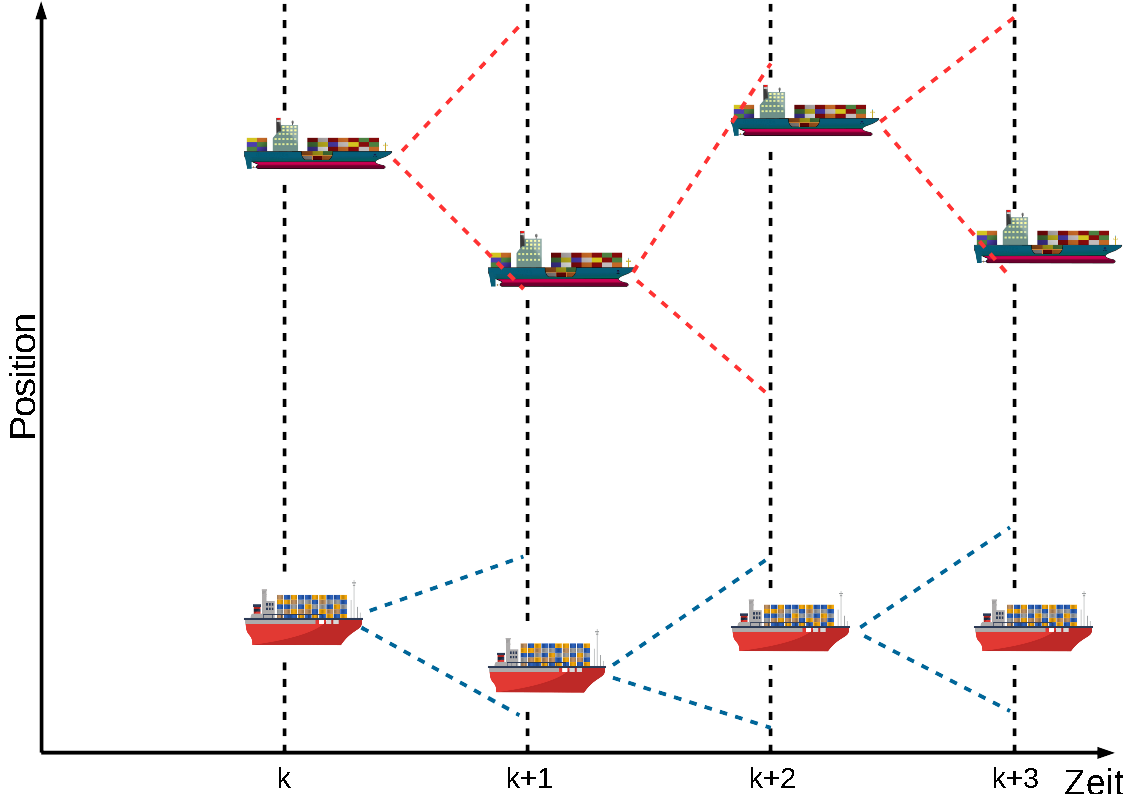
\includegraphics[width=0.7\linewidth]{./Pictures_report/Verhalten des Objekts.png}
		\caption{Verhalten des Objekts}
		\label{fig: Verhalten des Objekts}
	\end{figure}
	Diese unterschiedlichen Beständigkeiten können für die \textit{M/N-Logik} genutzt werden. Weiterhin ist zu erwähnen, dass die Qualität des Tracks bei diesem Algorithmus nur eine untergeordnete Rolle spielt. Es wird nur darauf Wert gelegt, dass die Messpunkte im nächsten Zeitschritt sich im entsprechenden Bereich befinden. 
	\newline
	Anhand dieser Ausgangssituation besteht die Aufgabe des Algorithmus darin die Anzahl der erfolgreichen Detektionen \textit{M} zu zählen, die innerhalb einer festen Anzahl an Scans \textit{N} vorkommen. Jeder Scan nimmt dabei einen Zeitschritt in Anspruch. Als erfolgreich wird eine Detektion eingestuft, wenn die Messpunkte von zwei Zeitschritten miteinander in Verbindung gebracht werden können,d.h. wenn es einen Messpunkt gibt, der sich im nächsten Zeitschritt in einem Gültigkeitsbereich befindet (Abbildung \ref{fig: Verhalten des Objekts}). Liegen keine passenden Messpunkte vor, so wird dies als Fehldetektion gewertet. Wird die Mindestanzahl \textit{M} an erfolgreichen Detektionen erreicht, liegt ein Objekt vor. Werden am Ende der \textit{N} Scans nicht ausreichend viele Detektionen erreicht, handelt es sich  wahrscheinlich nicht um ein Objekt, sondern um Messpunkte die durch Clutter verursacht wurden.
	\newline
	Zu diesem Zweck wird der Status eines Tracks (bestätigt, vorläufig, vernachlässigt) eingeführt. Ein Track gilt als bestätigt, wenn mindestens \textit{M} mal innerhalb von \textit{N} Scans das Objekt detektiert wurde. Wenn keine Möglichkeit besteht diese Häufigkeit zu erreichen, kann der Track vernachlässigt werden. Messpunkte, die der Algorithmus noch verarbeitet, sind als vorläufige einzustufen, weil sie nicht die Bedingungen erfüllen um als bestätigt oder vernachlässigt zu gelten. Abbildung \ref{fig: Status des Tracks} veranschaulicht welchen Status ein Track während des Algorithmus annehmen kann am Beispiel einer \textit{3/4-Logik} (3 benötigte Detektionen aus 4 Scans).
\begin{figure}[h]
		\centering
		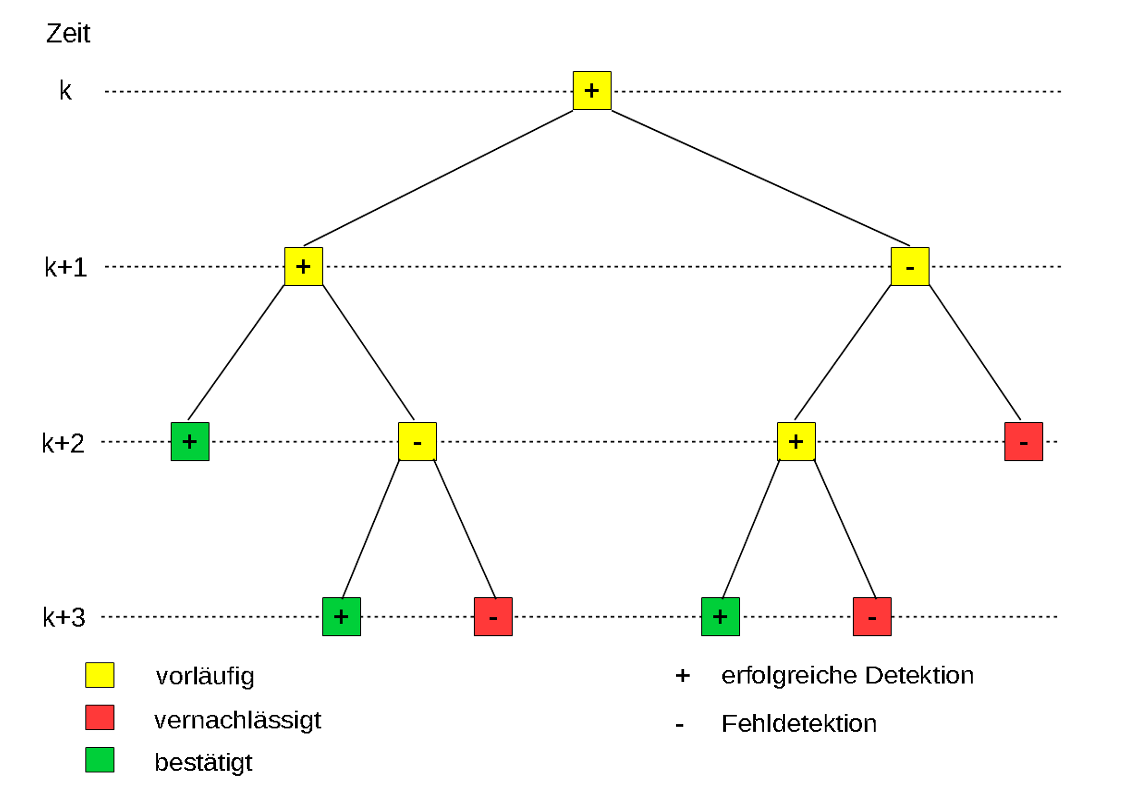
\includegraphics[width=0.7\linewidth]{./Pictures_report/Status des Tracks.png}
		\caption{Status des Tracks}
		\label{fig: Status des Tracks}
	\end{figure}
\subsection{Schwächen der M/N-Logik}
	Zwei Szenarien muss man immer beachten, wenn die \textit{M/N-Logik} genutzt wird. Erstens kann es bei der Messung dazu kommen, dass nicht nur sehr viel Clutter auftritt, sondern diese während der Messzeit so angeordnet sind wie Objekte, d.h. der Clutter ist sehr beständig. In diesem Fall wird die Anzahl der Objekte überschätzt.
	\newline
	Das zweite Szenario verursacht eine Unterschätzung der Objektanzahl. Dies wird hervorgerufen, wenn sich die Messdaten der Zielkörper unbeständig verhalten. Mögliche Gründe dafür sind häufig vorkommende Fehldetektion, tatsächliche Objekte die sich sehr schnell bewegen und gleichzeitig ihre Geschwindigkeit ändern. Letzteres spielt für diese Arbeit ein untergeordnete Rolle.
\subsection{Umsetzung}
	Dieses Unterkapitel befasst sich mit der Umsetzung des Algorithmus für das Projekt. Im folgenden werden die Wahl von \textit{M} und \textit{N}, eine grobe Implementierung und die Festlegung Gültigkeitsbereichs, um Objektmesspunkte von Clutter zu unterscheiden, vorgestellt. 
\subsubsection{Wahl von M und N}
	Bei der Entscheidung für ein passendes \textit{M/N}-Verhältnis sind Faktoren wie Realisierbarkeit, Qualität des Ergebnis und Rechenaufwand bzw. Rechendauer von großer Bedeutung. Hierfür ist eine Eingrenzung von $1/2<M/N<1$ sinnvoll, dabei sind \textit{M} und \textit{N} natürliche Zahlen. Die Anzahl an erfolgreichen Detektionen \textit{M} muss auf jeden Fall kleiner sein als die Scan-Häufigkeit. Der Grund hierfür ist, dass eine hundertprozentige Detektionsrate unrealistisch ist und der Algorithmus zu viele Messpunkte als Clutter einstufen würde. Den gegenteiligen Effekt, Clutter wird als Objekt behandelt, würde man erhalten, wenn \textit{M/N} zu niedrig ist. Mit einer \textit{2/3-Logik} erhält man einen Algorithmus mit minimaler Rechenzeit für eine schnelle Abschätzung, allerdings auf Kosten der Qualität. Mit größer werdendem \textit{M/N}-Verhältnis wird das Ergebnis genauer, jedoch stellt man erfahrungsgemäß fest, dass ab $N=5$ (\textit{4/5-Logik}) keine signifikante Verbesserungen auftreten, die eine weitere Erhöhung der Scan-Dauer bzw.-Anzahl rechtfertigen. Demzufolge ist die \textit{3/4-Logik} eine weiter Option mit einem qualitativ besseren Ergebnis. Für das Projektseminar hat man sich für $M=3$ und $N=4$ entschieden, weil bei einer maritimen Hinderniserfassung eine sehr schnelle Objektabschätzung nicht zwingend nötig ist und man mehr Wert auf die Qualität gelegt hat.
\subsubsection{Implementierung}
	Die grundlegend Struktur der \textit{M/N-Logik} kann wie folgt implementiert werden.
	\begin{algorithm}
	\caption{M/N-Algorithmus}
	\begin{algorithmic}[1]
	\State Initialisieren:
	\State $n_k=0$ (Anzahl der Objekte) 
	\State$m_k=1$ (Detektionen)
	\State$mbar=0$ (Fehldetektionen) 
	\State  Entscheidung zum Zeitpunkt $k$
	\For{alle vorläufigen Tracks}
		\If{Messpunkt im Gültigkeitsereich}
			\State $m_k\leftarrow m_k+1$			
		\Else{} (Keine Messpunkte im Gültigkeitsereich)
			\State $mbar\leftarrow mbar+1$
		\EndIf
		\If {$m_k \geq M$} (d.h. ausreichend Detektionen)
			\State Bestätige Track als Objekt
			\State $n_k\leftarrow n_k+1$
		\ElsIf{$mbar\geq N-M$} (d.h. zu viele Fehldetektionen)
			\State Vernachlässige Track
		\Else
			\State Fortfahren
		\EndIf		
	\EndFor
	\end{algorithmic}
	\end{algorithm}
	\newline
	Für die Startwerte des \textit{GNN} wurde der Algorithmus etwas modifiziert. Anstatt vom aktuellen Zeitpunkt ausgehend einen passenden Messpunkt im nächsten Zeitschritt zu finden, wie es in Abbildung \ref{fig: Verhalten des Objekts} der Fall ist, soll die \textit{M/N-Logik} zum Zeitpunkt $k$ in den vergangenen Messwerten die passenden Daten ermitteln. Abbildung \ref{fig: Rueckwaertslaufende Suchrichtung der MNLogik} zeigt das prinzipielle Vorgehen der rückwärts laufenden Suche.
	\begin{figure}[h]
	\centering
	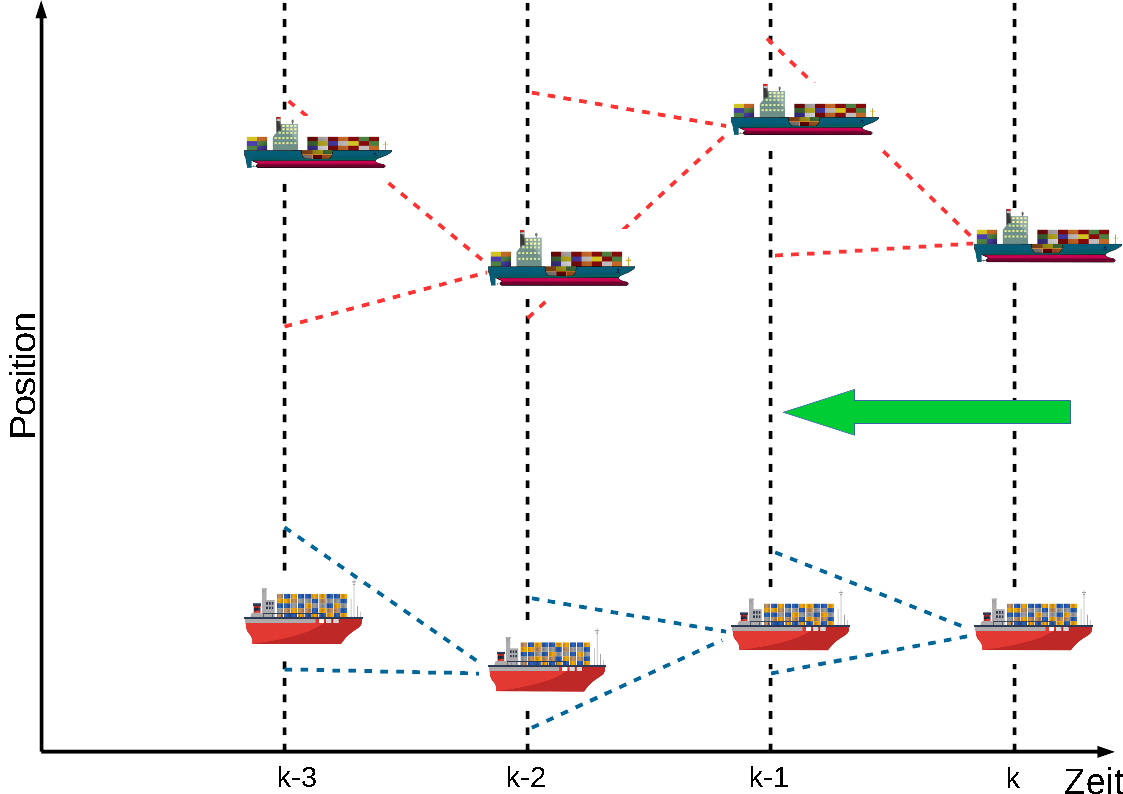
\includegraphics[width=0.7\linewidth]{./Pictures_report/Rueckwaertslaufende Suchrichtung der MNLogik.png}
	\caption{Rückwärtslaufende Suchrichtung der \textit{M/N-Logik}}
	\label{fig: Rueckwaertslaufende Suchrichtung der MNLogik}
	\end{figure}	
	Der Grund für diese Modifikation ist, dass dadurch die Ermittlung der Startwerte für den \textit{GNN-Algorithmus} vereinfacht wird. Man übernimmt die Koordinaten eines Tracks zum aktuellen Zeitpunkt $k$, das als Objekt bestätigt wurde und übergibt sie dem \textit{GNN}. Bei einer vorwärtslaufenden \textit{M/N-Logik} besteht die Möglichkeit, dass man am Ende mehrere Kandidaten pro Track bzw. Objekt hat und somit ein weiterer Algorithmus für die Auswahl der Anfangswerte nötig wäre.
\subsubsection{Gültigkeitsbereich}
	Der Gültigkeitsbereich wird genutzt, um darüber zu entscheiden ob eine erfolgreiche oder fehlgeschlagene Detektion vorliegt. Unter der Annahme, dass die Geschwindigkeiten bekannt sind, gilt der Zusammenhang
	\begin{equation}
		x_{k-1}=x_k-Tv^x_{k-1}
	\end{equation}
	\begin{equation*}
		y_{k-1}=y_k-Tv^y_{k-1}.
	\end{equation*}
	\newline
	Allerdings sind diese während der ersten $N$ Zeitschritte, dem sogenannten Warmlaufen, nicht gegeben, weshalb Anfangs nicht auf die Geschwindigkeiten zurück gegriffen werden kann um einen Gültigkeitsbereich zu bestimmen. Stattdessen musste über die Koordinaten der Messdaten eine Schwelle für diesen Bereich ermittelt werden. Als Bedingung für die Gültigkeit wurde eine Umgebung $u$ mit
	\begin{equation}
		|z^x_k-z^x_{k-1}|\leq u
	\end{equation}
	\begin{equation*}
		|z^y_k-z^y_{k-1}|\leq u
	\end{equation*}
	\newline
	festgelegt, die den maximalen Abstand zweier Messpunkte angibt. $z^x$ bzw. $z^y$ beschreibt hierbei die $x$- bzw. $y$-Koordinate eines Messpunktes. Ist der Abstand zwischen den Messpunkten ausreichend klein ($z_{k-1}$ liegt also im Gültigkeitsbereich), kann dies als eine erfolgreiche Detektion gewertet werden. Welcher Wert für $u$ genommen wird, hängt von der Anwendung selbst ab und musste durch Trail-and-Error herausgefunden werden. Dazu wurden die Messdaten, bezogen auf die maximal und minimal Wert der Koordinaten, durch
	\begin{equation}
		z^x_{norm}=\cfrac{z^x-x_{min}}{x_{max}-x_{min}}
	\end{equation}
	\begin{equation*}
		z^y_{norm}=\cfrac{z^y-y_{min}}{y_{max}-y_{min}}
	\end{equation*}
	\newline
	normiert, um alle Daten auf die gleiche Größenordnung zu bringen. Dadurch wird das Ermitteln eines passenden $u$ deutlich erleichtert. Nach dem der \textit{M/N-Algorithmus} die Messdaten verarbeitet hat, erfolgte eine Rücktransformation mit
	\begin{equation}
		z^x=(x_{max}-x_{min})z^x_{norm}+x_{min}
	\end{equation}
	\begin{equation*}
		z^y=(y_{max}-y_{min})z^y_{norm}+y_{min}.
	\end{equation*}
	\newline
	Nach den ersten $N$ Zeitschritten kann der \textit{GNN-Algorithmus} die Geschwindigkeiten der Objekte schätzen. Diese Schätzungen wurden für den Rest der Simulation genutzt um einen genaueren Gültigkeitsbereich zu bestimmen. Mit dem Zusammenhang
	\begin{equation}
		\hat{x}_{k-1}=z^x_k-T\hat{v}^x_{k-1}
	\end{equation}
	\begin{equation*}
		\hat{y}_{k-1}=z^y_k-T\hat{v}^y_{k-1}
	\end{equation*}
	\newline
	kann geschätzt werden, wo sich mögliche Messpunkte befinden. Als Schwelle  für den Gültigkeitsbereich wurde der Fehlertoleranz $\epsilon$ mit
	\begin{equation}
		|z^x_{k-1}-\hat{x}_{k-1}|\leq \epsilon
	\end{equation}
	\begin{equation*}
		|z^y_{k-1}-\hat{y}_{k-1}|\leq \epsilon
	\end{equation*}
	\newline
	definiert. Ist der Fehler ausreichend klein, dann liegt $z_{k-1}$ im Gültigkeitsbereich und man kann von einer erfolgreichen Detektion aus gehen. Für die Bestimmung von $\epsilon$ musste man auch hier nach Trail-and-Error vorgehen. Die Normierung wurden ebenfalls wie oben durchgeführt.


\subsection{Startwerte}
Die Genauigkeit der Zustandsschätzung des GNN ist von der Wahl der Positionsstartwerten stark abhängig. Bild \ref{pic:GNNSW} veranschaulicht diesen Performance Unterschied anhand  Testdaten. \\


\begin{figure}[h!]\label{pic:GNNSW}
    \centering
    \begin{subfigure}{0.6\textwidth}
        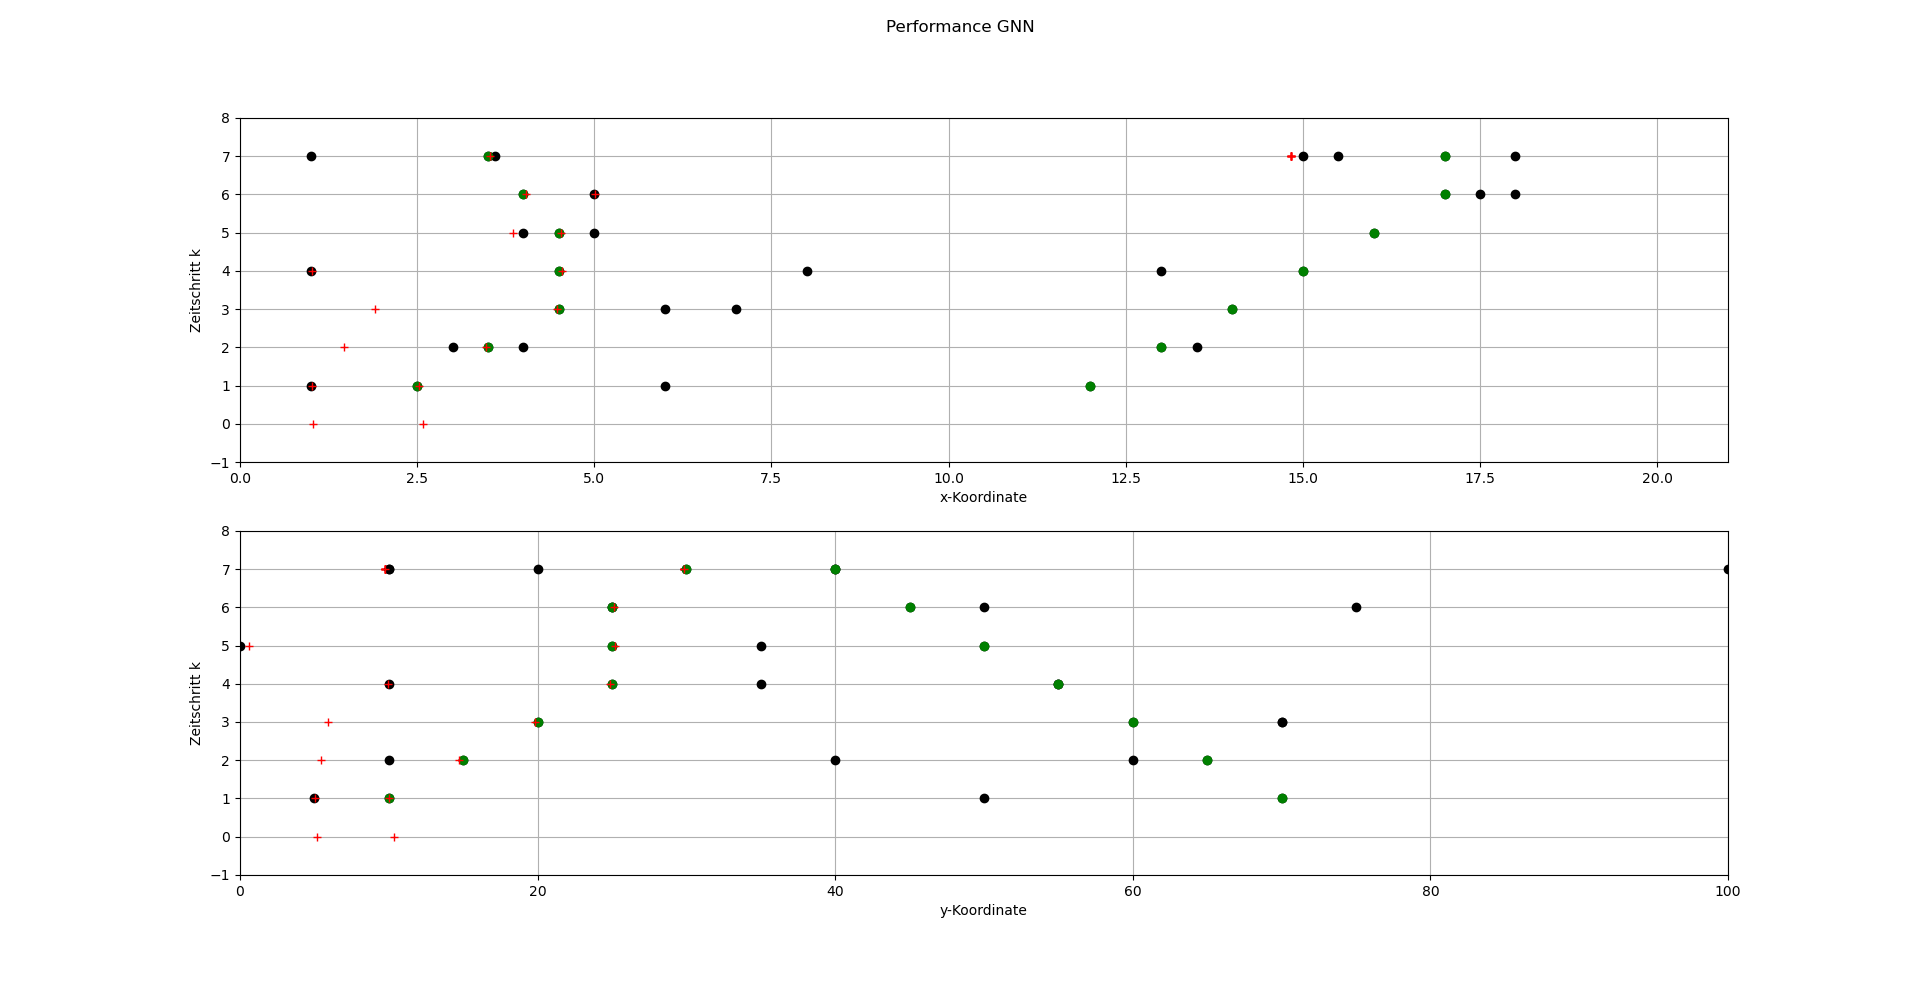
\includegraphics[width=13cm]{./Pictures_report/GNNTestdatenSW0.png}
        \subcaption{x,y Schätzung anhand ungeeigneter Startwerten. Ein von zwei Objekt richtig erkannt}
    \end{subfigure}

\medskip
    \begin{subfigure}{0.6\textwidth}
        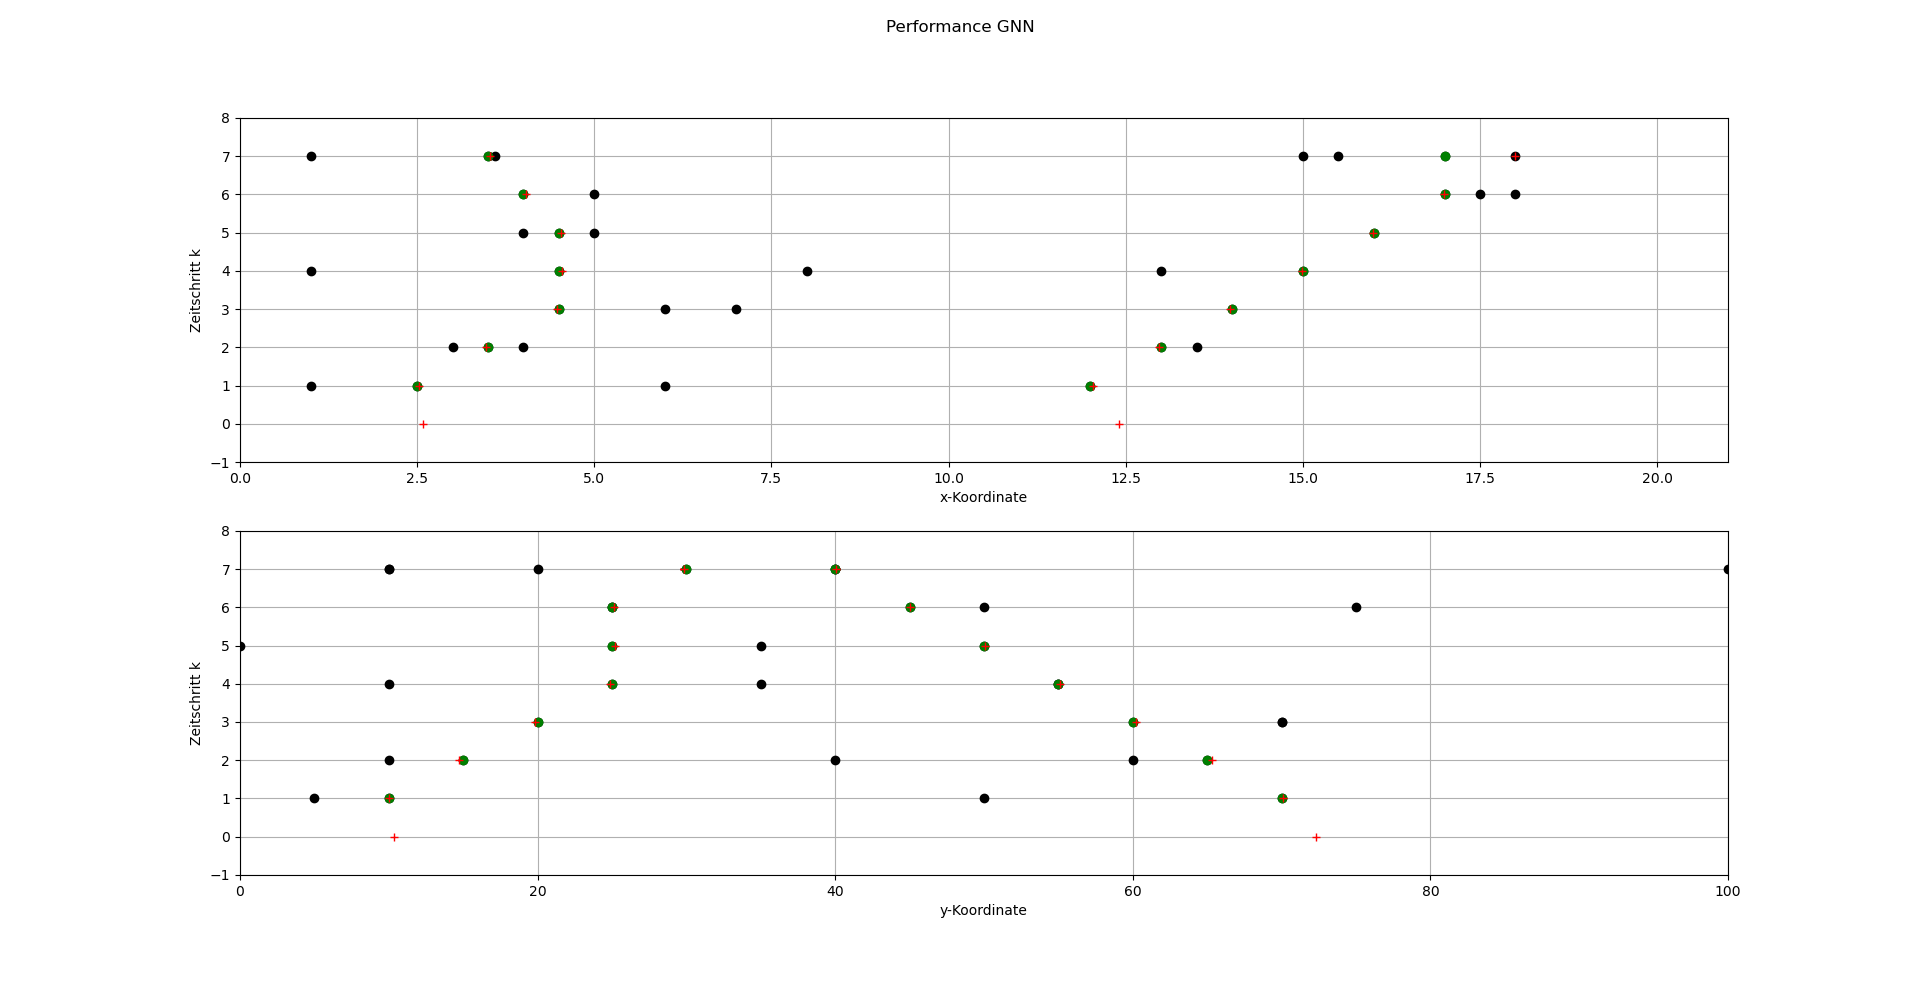
\includegraphics[width= 13cm]{./Pictures_report/GNNTestdatenSW1.png}
        \subcaption{x,y Schätzung anhand geeigneter Startwerten. Beide Objekte richtig erkannt}
    \end{subfigure}
    \caption[]{GNN Performance, mit geeigneten und ungeeigneten Startwerte und $n_k = const. = 2$. Die schwarze Punkte repräsentiert die Clutters, die grüne die echte Positionen der Objekten und die rote Kreuze stellen die geschätzten Positionen des GNN dar }
    \label{pic:GNNSW}
\end{figure}


Die Platzierung der Startwerten entscheidet also, ob die Schätzung des GNN als sehr gut oder als sehr schlecht eingestuft werden kann, was den Einsatz des Algorithmus in Frage stellen kann. Aus dem Grund, nutzt man die Zeitverzögerung, die bereits für die Anwendung des \textit{M/N Algorithmus} erforderlich ist, um genaueren Startwerten aus den Messungen zu extrahieren.\\
Nach der Bestimmung der Objektanzahl, analysiert der \textit{M/N Algorithmus} welche Koordinaten welchem Objektkandidaten gehört und diese werden als x,y Größe für den Zeitschritt $k = N-1$ verwendet. Werden die richtige Objektkandidaten gefunden, kann man sicherstellen, dass die Startwerte geeignet sind. Falls die gefundenen Kandidaten sich mit den echte unterscheiden, liegen die Startwerte auch falsch und die Qualität der Schätzung des GNN wird je stärker beeinträchtigt je größer diese Abweichung ist.\\
Die Anfangsgeschwindigkeiten $v^x$ und $v^y$ werden immer als null initialisiert.
\subsection{Deaths and Births}\label{subsub:GNNDeathBirth}
In einem praktischen Anwendungsszenario bleibt selbstverständlich die Anzahl der Objekte nicht konstant. Daher in jedem Zeitschritt wird es eine Analyse benötigt, die entscheidet ob ein neues Objekt auf die Bildaufnahme aufgetreten oder verschwunden ist. Man nennt solches Verfahren als \textit{Deaths and Births Analyse}.\\
Zum Gegenteil des \textit{PHD- Algorithmus} wird dieser Schritt bei dem \textit{GNN } simpel gehalten. Nach der Bestimmung der Objektanzahl $n_k$, ist ein Objekt \textit{gestorben}, falls $n_k < n_{k-1}$ und wurde \textit{geboren}, falls $n_k > n_{k-1}$.\\
Für den ersten Fall, vergleicht man die Positionen der Objekte anhand der $k$ und $k-1$ Zeitschritten. Die Koordinaten aus $k-1$, die betragsmäßig am weitesten der neuen Koordinaten $k$ liegen, werden aus dem Zustand gelöscht, daher Objekte, die diesen Koordinaten entsprechen werden als \textit{Tot} angesehen. Die Kovarianzmatrix des Schätzfehlers, die dem gelöschten Zustand gehört wir ebenfalls nicht weiter berücksichtigt. \\
Für den Fall neuer Geburten, vergleicht man wieder die Beträge der Position über den letzten zwei Zeitschritten. Die Objekte dessen Koordinaten auf $k-1$ die größten Abstände zum $k$ aufweisen, werden als Objekte, die neulich geboren wurden, erkannt. Deren Positionen werden zusammen mit den Anfangsgeschwindigkeiten in den aktualisierten Zustand eingespeichert. Die Kovarianzmatrix des Schätzfehlers neuer Objekte werden mit $\textbf{P}^i_0$ initialisiert.
\newline
\newline
\section{\textit{GNN} Zusammenfassung}
Nach der Vorstellung des Aufbaus des \textit{Algorithmus}, ist es möglich seine komplette Struktur darzustellen.\\
\begin{algorithm}
\caption{GNN Algorithmus - Pseudocode}
\label{alg:GNNAlgorithm}
\begin{algorithmic}[1]
\State Initialisieren: $n_k = -1$, $k = 0$
\While{Bilder vorhanden}
  \State Koordinaten vom Zeitschritt $k$ aus der Detektion erhalten
  \State Messungsanzahl $m_k$ aus den Koordinaten
  \If{$k < N$ }
  \State Messungen für \textit{M/N Algorithmus} laden
  \EndIf
  \If {$k = N$ }
  \State $n_k$ aus dem \textit{M/N Algorithmus}
  \State Initialisierung $\underline{x}_{N|N-1}$
  \EndIf
  \If {$k>N$}
      \For{$i \leq n_k$}
          \State \textit{Kalman-Prädiktion: }$\underline{x}_{k|k-1}$ und $\textbf{P}_{k|k-1}$  mithilfe der Gleichungen  \ref{eq:GNNPraediktionX} und                 \ref{eq:GNNPraediktionP} ausrechnen .
          \State Kostenmatrix mithilfe der Gleichung \eqref{eq:GNNKostenMatrix} erstellen 
          \State Wahrscheinlichste Hypothese mithilfe eines \textit{Hungarian-Algorithmus}
          \State \textit{Kalman-Update: }$underline{x}_{k|k}$ und $\textbf{P}_{k|k}$ mithilfe der Gleichungen \ref{eq:GNNUpdate} korrigieren
          \State $underline{x}_{k|k}$ ausgeben
      \EndFor
      \State Daten für \textit{M/N Algorithmus} aktualisieren
      \State $n_{k+1}$ bestimmen mithilfe des  \textit{M/N Algorithmus}
      \State $\underline{x}_{k+1|k}$ und $\textbf{P}_{k+1|k}$ mithilfe \textit{Deaths and Births Analyse} ergänzen
      
  \EndIf
  $k = k+1$
\EndWhile


\end{algorithmic}
\end{algorithm}

\section{Ergebnisauswertung auf Testdaten}\label{sub:GNNEinflussParam}
Wie bereits auf Bild \ref{pic:GNNSW} gezeigt, findet der \textit{GNN} das richtige Tracking anhand der Testdaten lediglich, wenn der Startwert den echten Positionen annähert. Bild \ref{pic:GNNXY} zeigt die Schätzung der x,y Koordinaten. Man beobachte, dass in der Regel, die Zustände beider Objekte nur einen geringen Fehler aufweisen. Der Erfolg der Schätzung kann hauptsächlich der Tatsache zugewiesen werden, dass die Clutters sich nicht wie die angenommene Bewegung der Objekten (\textit{Constant Velocity Model}) bewegen. Außerdem, findet weder ein \textit{Birth} noch ein \textit{Death} statt und letztlich sind die Hyperparameter genau auf diese Problematik angepasst. In einer praktischen Umwelt sind diese Vereinfachungen allerdings meistens nicht erfüllbar. Eine Performanceanalyse hinsichtlich praxisorientierter Datensätze wird im Kapitel \ref{.} zusammen mit der Performance des \textit{PHD-Filter} vorgestellt.  \\
\begin{figure}[h!]
\begin{center}
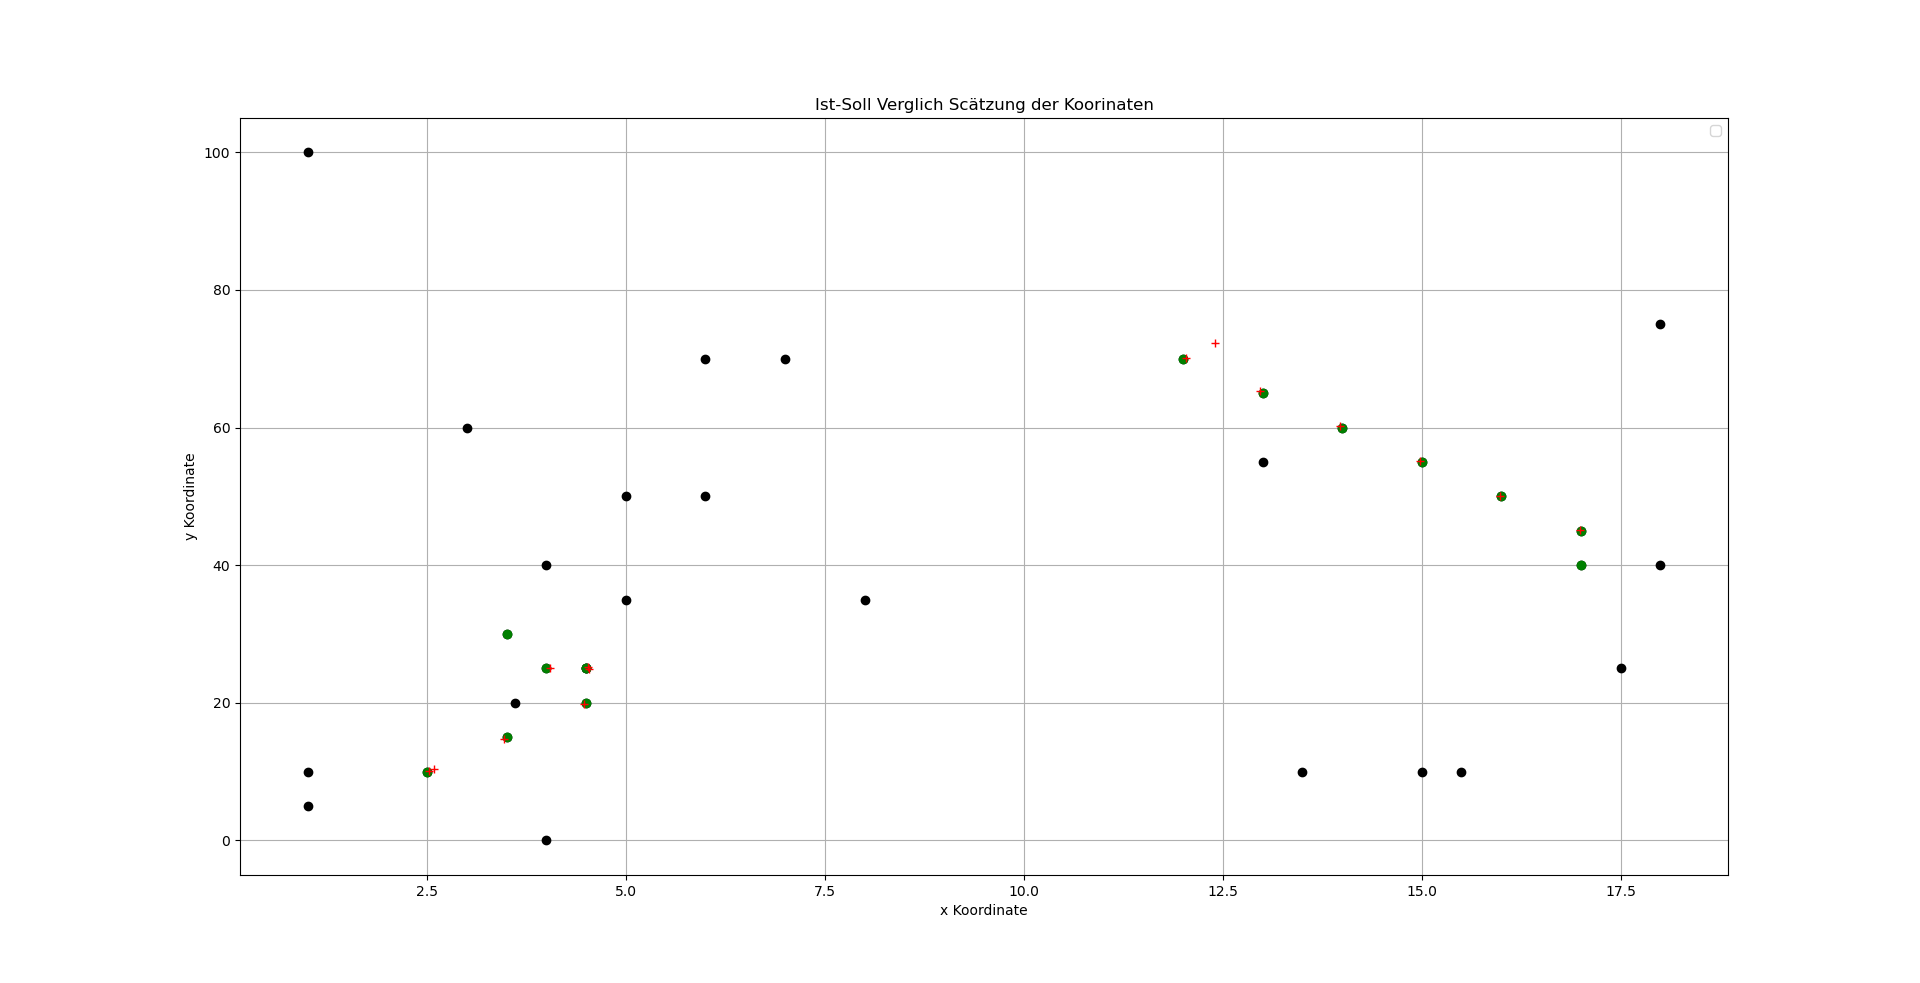
\includegraphics[width=12 cm]{./Pictures_report/GNNTestdatenXY}\label{ConvexConcave}
\caption{Ist-Soll Vergleich der Koordinatenschätzung: Die schwarze Punkte repräsentiert die Clutters, die grüne die echte Positionen der Objekten und die rote Kreuze stellen die geschätzten Positionen des GNN dar}
\label{pic:GNNXY}
\end{center}
\end{figure}

Die erforderliche Hyperparameter, die diese Schätzung erzeugt habe, sind folgendermaßen dargestellt.\\
\begin{itemize}
  \item $\textbf{Q} = \begin{bmatrix}
10 &0 &0&0&0 \\
0 &10 &0&0&0\\
0 &0 &10&0&0\\
0 &0 &0&0&10\\
\end{bmatrix}$
  \item $\textbf{R} = \begin{bmatrix}
1 &0  \\
0 &1\\
\end{bmatrix}$
  \item $\textbf{P}_0 = \begin{bmatrix}
100 &0 &0&0 \\
0 &1 &0&0\\
0 &0 &100&0\\
0 &0 &0&1\\
\end{bmatrix}$
   \item $M = 4$
   \item $N = 5$
   \item $p^D = 0.99$
   \item $\eta = 0.08$
\end{itemize}
Kapitel \ref{subsub: GNNParameter} beschäftigt sich mit der Variation dieser Parameter und wie sie den Algorithmus beeinflusst.\\

\subsection{Einfluss der Hyperparametern}\label{subsub: GNNParameter}
Bild \ref{pic:GNNPD} zeigt wie eine leichte Verringerung der Detektionsrate $p^D$ bereits zu einer falschen Schätzung führen kann. Es liegt daran, der die $l_{i,0}$ Werte der Kostenmatrix, verglichen mit den $l_{i,j}$ kleiner werden. Infolgedessen wird die Wahrscheinlichkeit einer Nicht-Detektion gegenüber einer Detektion übergewichtet, daher werden die Werte von $\theta^*_k$ öfters gleich null sein und die Kalman-Korrektur reicht mehrmals die gleichen Werte der Prädiktion weiter, ohne die Schätzung anhand echter Messungen zu aktualisieren. \\
\begin{figure}[h!]
\begin{center}
\includegraphics[width=13 cm]{./Pictures_report/GNNPD}
\caption{Einfluss $p^D = 0.95$: Die schwarze Punkte repräsentiert die Clutters, die grüne die echte Positionen der Objekten und die rote Kreuze stellen die geschätzten Positionen des GNN dar}
\label{pic:GNNPD}
\end{center}
\end{figure}
Eine Vergrößerung oder Verkleinerung der Werten der Matrizen $\textbf{Q}$, $\textbf{R}$ und $\textbf{P}_0$ bedeutet eine $1000$-Faktor Multiplikation beziehungsweise Division von den gegebenen Matrizen aus dem letzten Kapitel.\\
Die Varianz des Modellrauschen $\textbf{Q}$ entscheidet über die Einsatzfähigkeit des Algorithmus. Je mehr Wissen man über die Startwerte und das Systemrauschen verfügt, desto kleiner müssen die Werte von $\textbf{Q}$ gewählt werden. Eine betragsmäßig höhere $\textbf{Q}$ erlaubt dem Kalman-Filter eine höhere Abweichung des Zustands über Zeitschritten hinaus, daher werden höhere \textit{Sprünge} ermöglicht, was sich für ein Szenario aneignet, wo weniger Wissen über die Anfangsbedingungen vorhanden ist. Bild \ref{pic:GNNQ0} veranschaulicht: wenn $\textbf{Q}$ zu gering gewählt wird, verringert sich erheblich die Reaktionszeit auf unerwartete Messungen des \textit{GNN}.\\
\begin{figure}[h!]
\centering
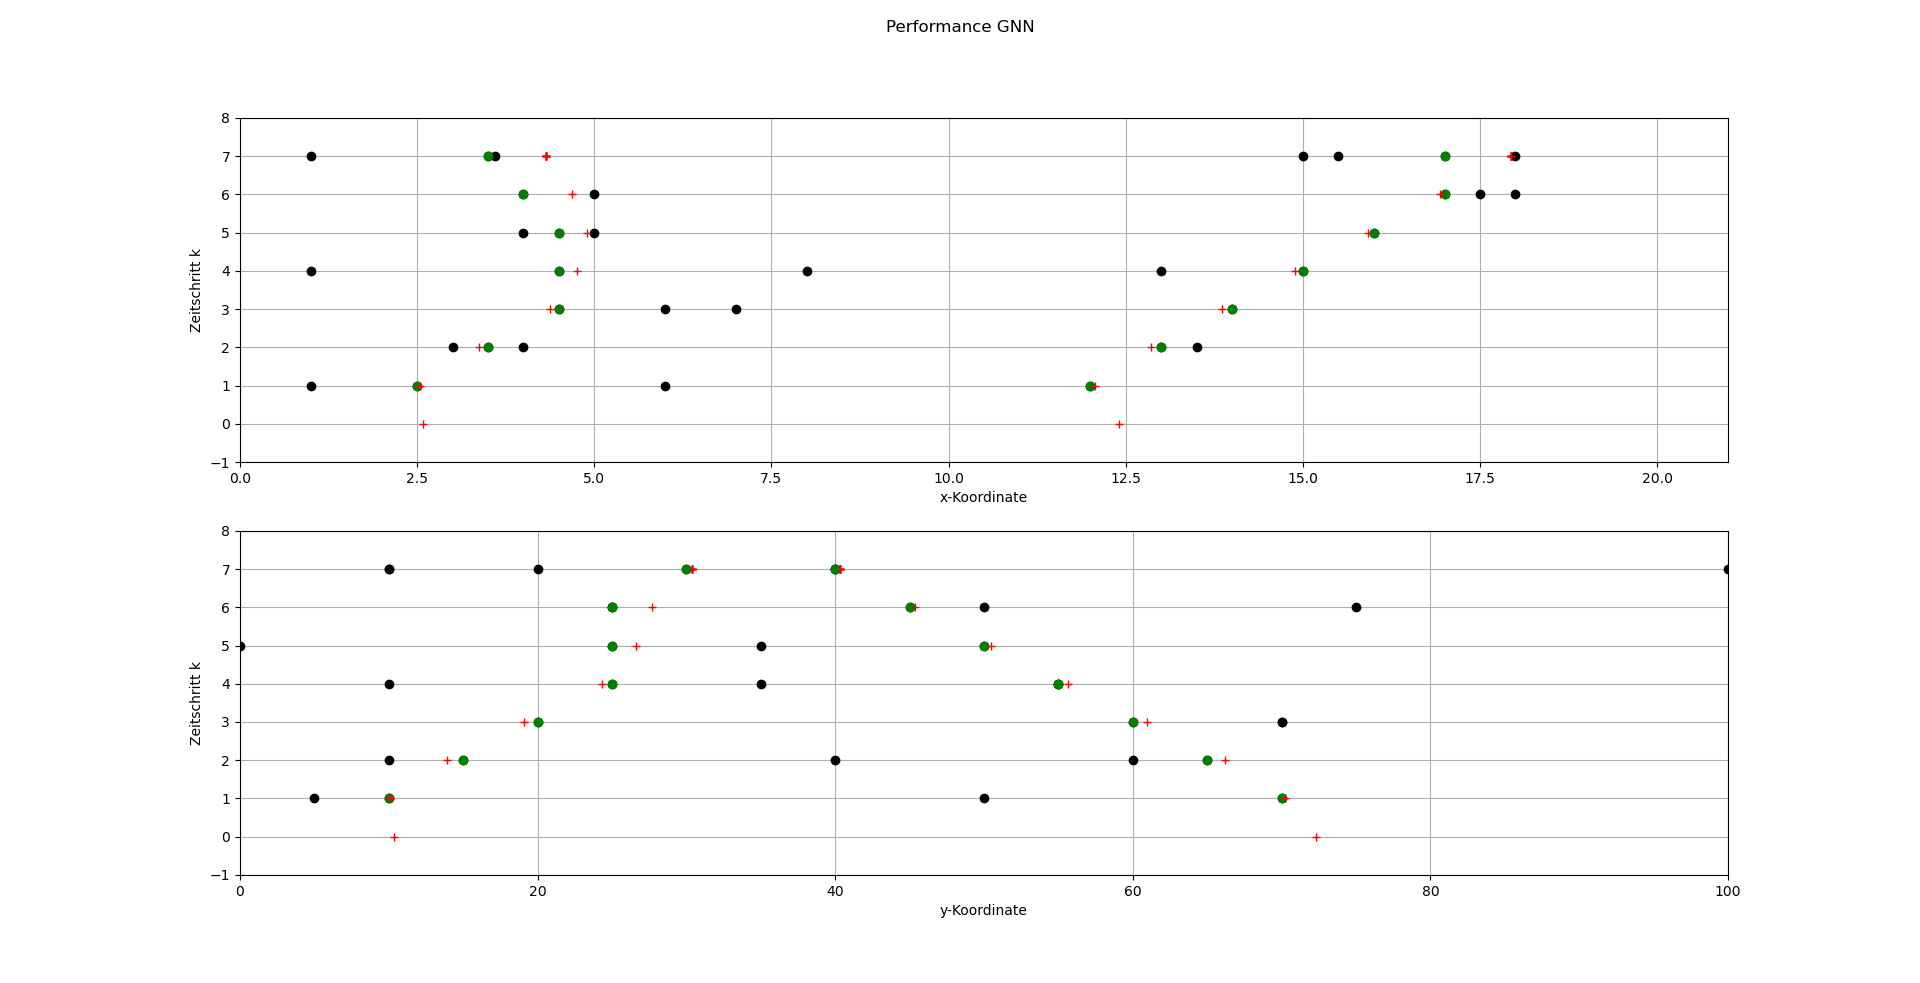
\includegraphics[width=12 cm]{./Pictures_report/GNNQ0}
\caption{Einfluss einer Verringerung der Werten von $\textbf{Q}$: Die schwarze Punkte repräsentiert die Clutters, die grüne die echte Positionen der Objekten und die rote Kreuze stellen die geschätzten Positionen des GNN dar}
\label{pic:GNNQ0}
%\end{center}
\end{figure}
Die Varianz des Messrauschens $\textbf{R}$ entscheidet wie stark der Algorithmus von den Messungen abhängig gestaltet wird. Je kleiner die Werte von dieser Matrix, desto geringerer ist die Abweichung der Schätzung bezüglich der Messungen. Dies führt zu einer Überanpassungsgefahr, da bei einer Clutter-behateten Umwelt, der unerwünschte Einfluss der Clutters übergewichtet wird. Allerdings für große $\textbf{R}$ Werte, wird der Einfluss der Messungen derart untergewichtet, dass der Algorithmus Schätzungen mit enormer Abweichung zur Realität suggeriert. Dieser Effekt wird genau auf Bild \ref{pic:GNNR1} erkannt, wo der Einfluss der Messungen nach wenigen Zeitschritten schon beinah vernachlässigt wird.\\
\begin{figure}[h!]
\centering
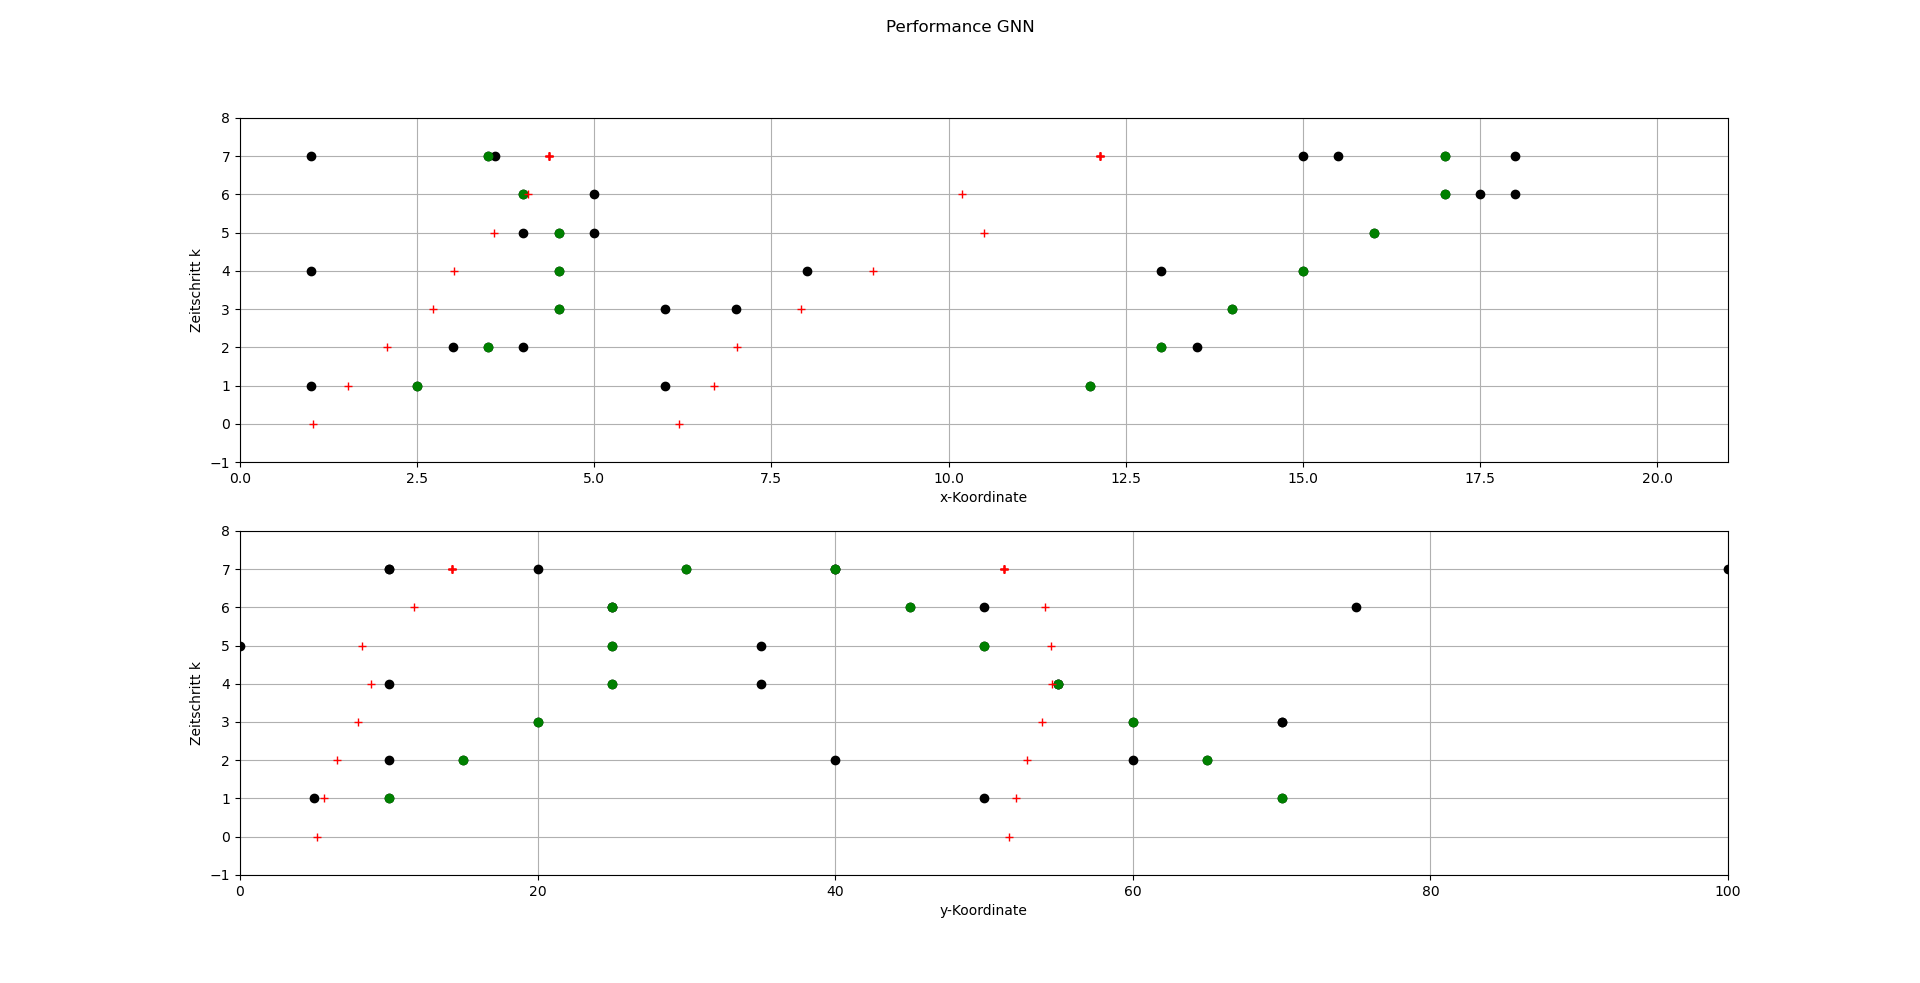
\includegraphics[width=12 cm]{./Pictures_report/GNNR1}
\caption{Einfluss einer Vergrößerung der Werten von $\textbf{R}$ : Die schwarze Punkte repräsentiert die Clutters, die grüne die echte Positionen der Objekten und die rote Kreuze stellen die geschätzten Positionen des GNN dar}
\label{pic:GNNR1}
%\end{center}
\end{figure}
Ähnlich wie bei der Wahl der Varianz des Modellrauschens, sind die Werte der Kovarianzmatrix des Schätzfehlers $\textbf{P}_0$ abhängig von dem Vorwissen des Anfangsbereichs. Ist kein Vorwissen vorhanden, werden höhere Werte von $\textbf{P}$ erforderlich, die noch das Tracking der Objekte ermöglichen. Da, man tatsächlich mithilfe der Zeitverzögerung, die für den \textit{M/N Algorithmus} erforderlich ist, Informationen über den Bereich der Anfangsbedingung erhält, empfiehlt \cite{IDS} diesen für die Wahl der $\textbf{P}_0$ zu nutzen. Bild \ref{pic:GNNP} zeigt die Qualitätsminderung für die Wahl ungeeigneter Anfangswerten von $\textbf{P}_0$.\\
\begin{figure}[h!]
    \centering
    \begin{subfigure}{0.6\textwidth}
        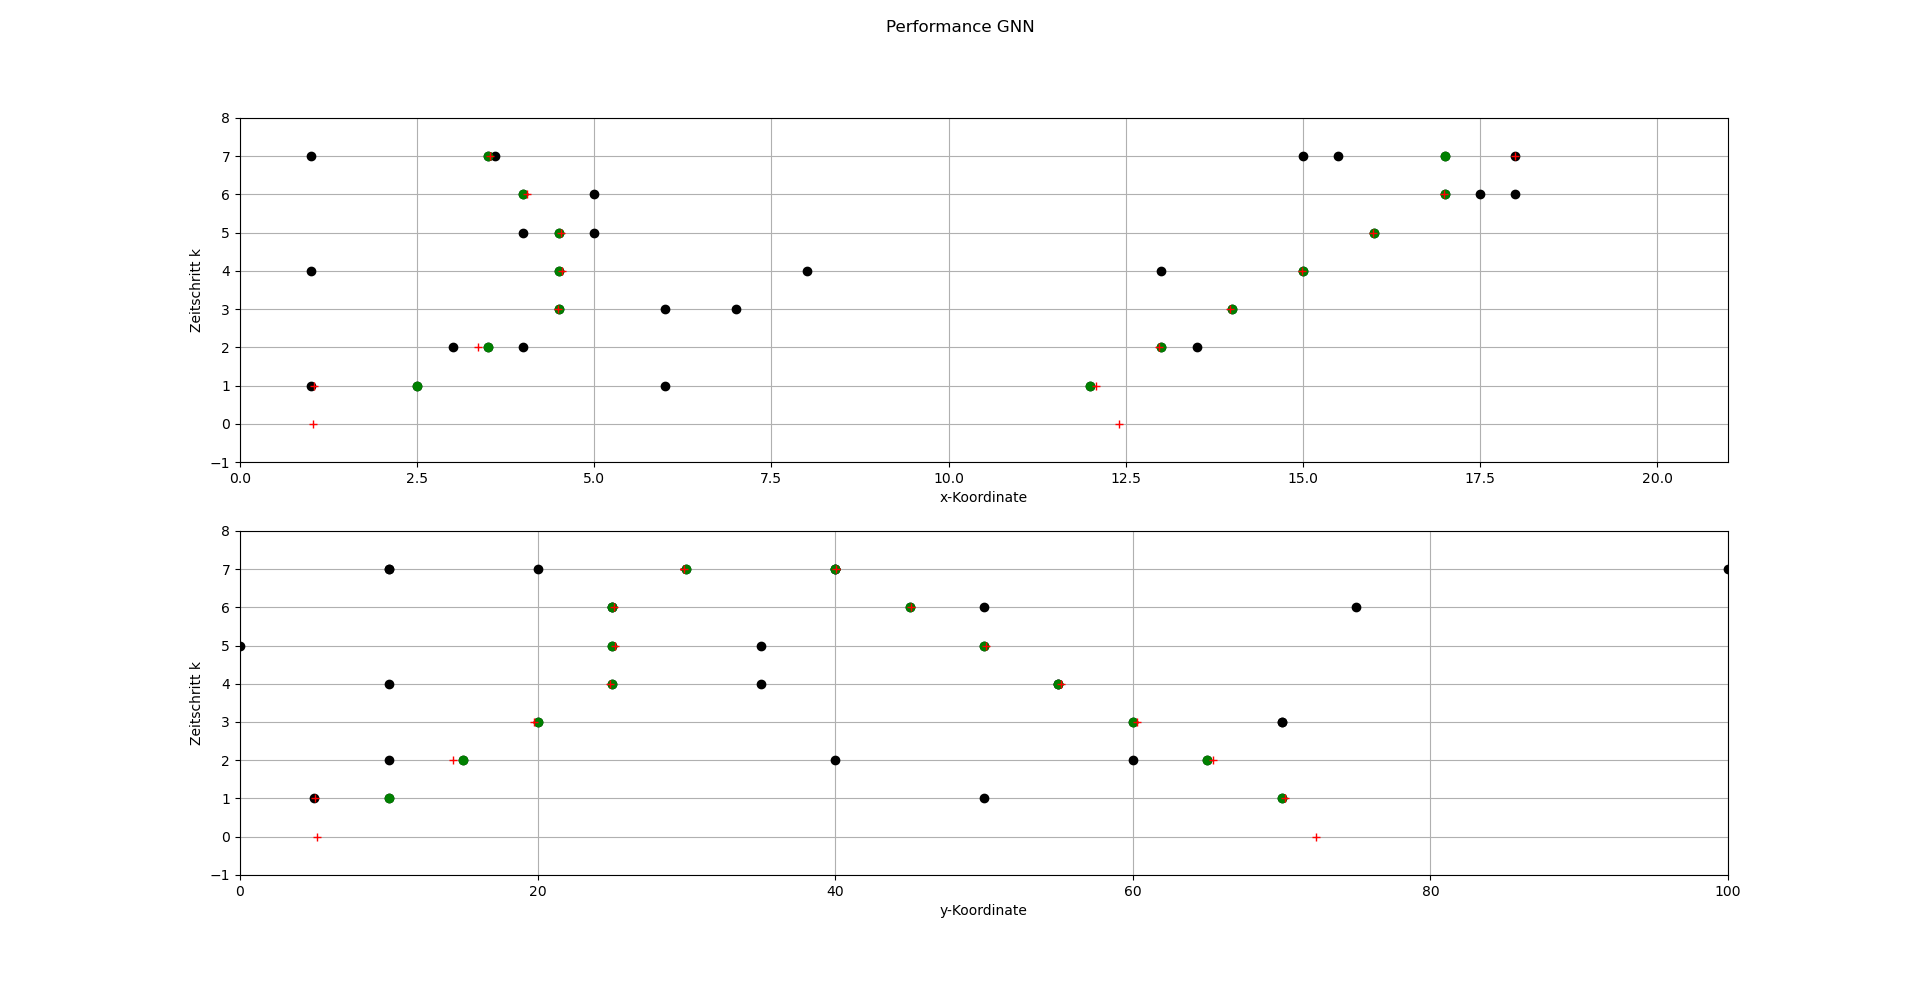
\includegraphics[width=11cm]{./Pictures_report/GNNP0.png}
        \subcaption{Einfluss einer Verkleinerung der Werten von $\textbf{P}_0$}
       % \label{pic:GNNSW0}
    \end{subfigure}

\medskip
    \begin{subfigure}{0.6\textwidth}
        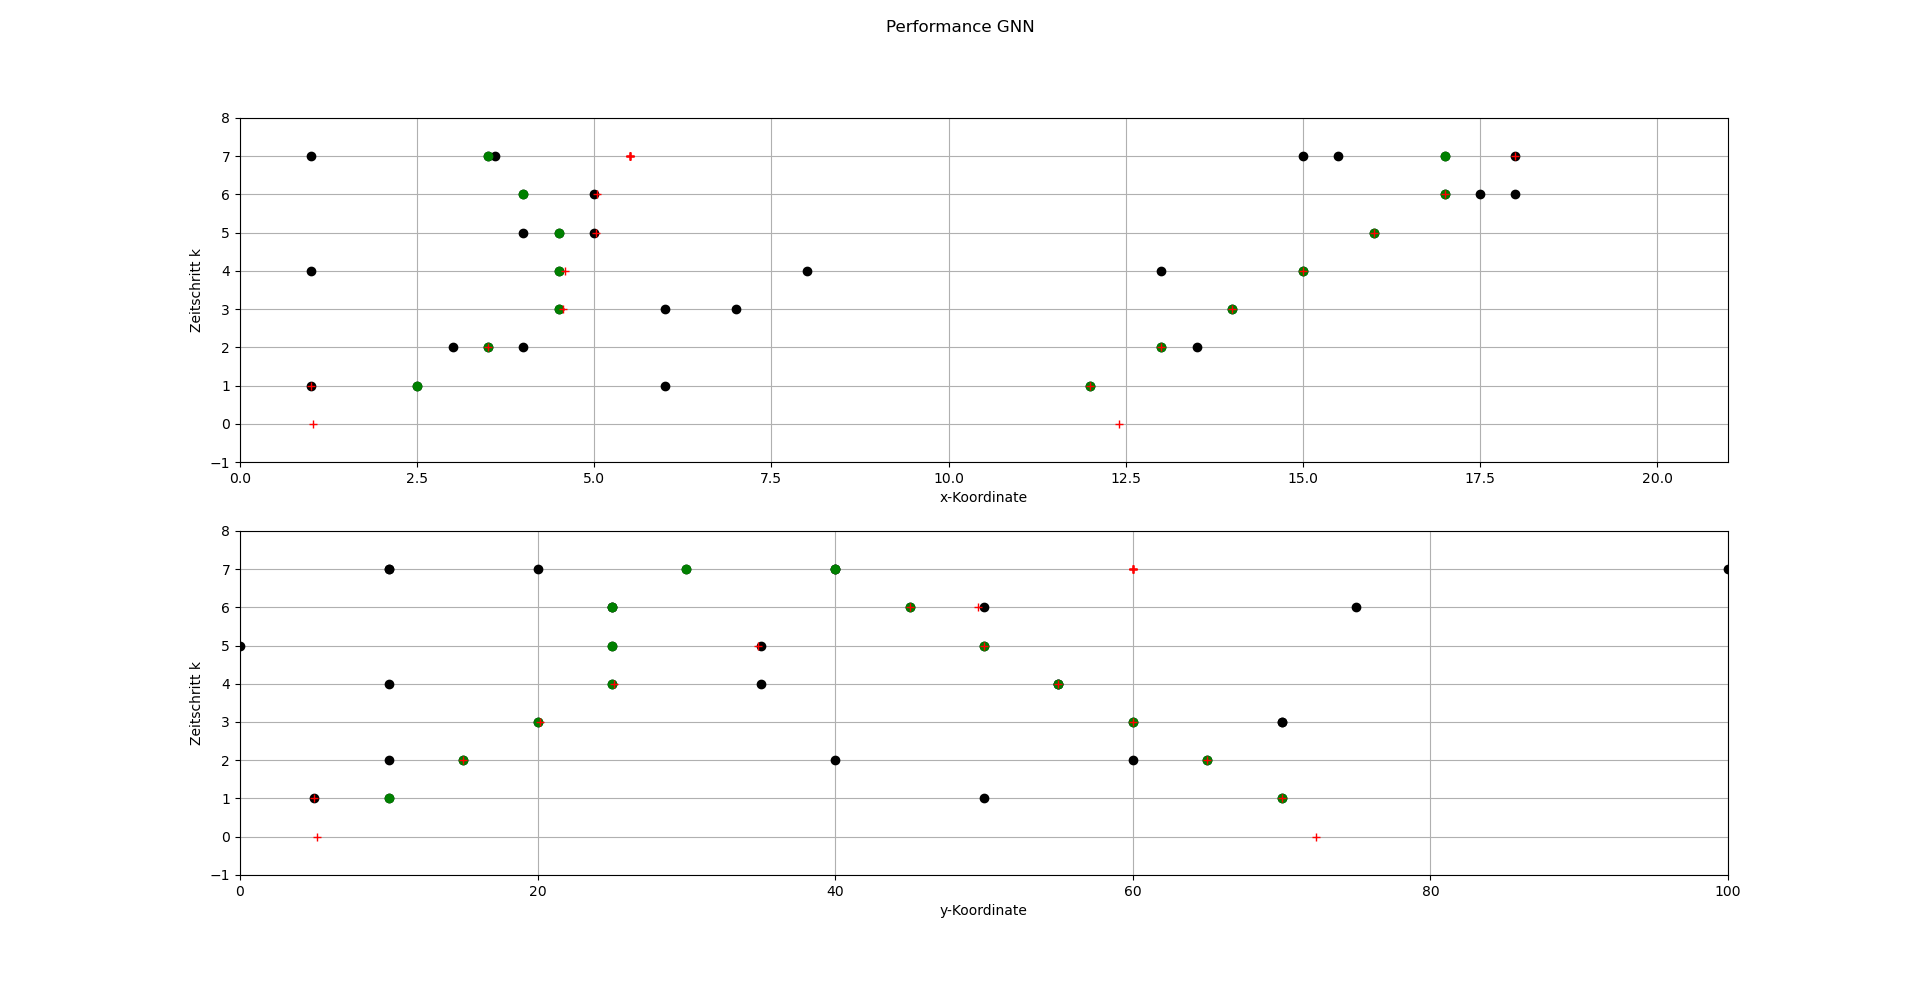
\includegraphics[width= 11cm]{./Pictures_report/GNNP1.png}
        \subcaption{Einfluss einer Vergrößerung der Weten von $\textbf{P}_0$}
        \label{fig:arm4}
    \end{subfigure}
    \caption[]{GNN Performance, mit unterschiedlichen Anfangswerten $\textbf{P}_0$. Die schwarze Punkte repräsentiert die Clutters, die grüne die echte Positionen der Objekten und die rote Kreuze stellen die geschätzten Positionen des GNN dar  }
    \label{pic:GNNP}
\end{figure}
\section{Einschränkung des Algorithmus}
Der Entwurf eines rechnengünstigen und schnellen Algorithmus wie der \textit{GNN} wird auf Kosten bestimmter Einschränkungen ausgelegt. Folgende Liste präsentiert ein Fazit über die Haupteinschränkungen und warum für bestimmte maritmischen Szenarien die Anwendung des \textit{GNN} problematisch sein kann.\\
\begin{itemize}
  \item \textit{GNN Prunning:} Die Berücksichtigung von lediglich der wahrscheinlichsten Datenassoziation ist der Grund warum der \textit{GNN} simpel uns schnell ist. Allerdings, es reichen wenige Zeitschritten, wo die wahrscheinlichste Hypothese nicht der Bewegung eines Objekts entspricht, um die Verfolgung dieses Objekts komplett zu unterbrechen. Eine maritmische Umwelt, wo viele Clutters vorhanden sind können den Einsatz dieses Algorithmus verhindern. Aus dem Grund, der Einsatz ist nur zu gerecht fertigen, wenn die Detektionsqualität als hoch eingestuft wird.
  \item Der Algorithmus geht prinzipiell von einer bekannten und konstante Objektanzahl aus. Damit man dies umgehen kann, integriert man den \textit{M/N Algorithmus} was nur eine grobe Einschätzung des $n_k$ abliefert. Außerdem, wird eine Zeitverzögerung von einigen Frames erforderlich, bevor der Zustand ausgegeben wird.
 \item \textit{Deaths and Births Model}. Dies ist ebenso ein wichtiges Element, das der \textit{GNN} prinzipiell nicht berücksichtigt. Anhand dieser Arbeit werden die Annahmen im Kapitel \ref{subsub:GNNDeathBirth} getroffen. Diese Annahmen können ebenfalls die Trackingsqualität verringern.
  \item \textit{Hohe Detektionsrate erforderlich:} Aufgrund der Auslegung der Gleichung der Kostenmatrix, wird eine hohe Detektionsrate erforderlich, damit der \textit{Hungarian Algorithmus} die Messung des Objekts nicht als eine Nicht-detektion einstuft. In der praktischen Anwendung bedeutet, dass eine hohe Kameraqualität erwünscht ist.
  \item \textit{Auswahl der Kalman-Filter Parametern:} Die Wahl der Varianzmatrizen des Kalman-Filters führen zu einer Überanpassungsgefahr an bestimmten Szenarien. Wenn die Umweltbedingungen sich viel unterscheiden von Bedingungen, an den die Parameter festgelegt wurden, werden die Ergebnisse von der Realität abweichen. Bei der Wahl dieser Parameter wird eine bestimmte Erfahrung des Benutzers erforderlich.
  \item \textit{Constant Velocity Model}: Dies ist eine Einschränkung die eigentlich alle Algorithmen, die von diesem Modell ausgehen, betrifft. Wenn Objekte sich mit einer großen Beschleunigung bewegen, wird deren Verfolgung stark beeinträchtigt. Außerdem, wenn Clutters nicht zufällig vorkommen, sondern sich näherungsweise konstant und linear "bewegen", werden die vermutlich als Objekt erkannt. 
\end{itemize}


\bibliographystyle{apacite}
\bibliography{Referenzen}
\end{document}
